\subsection{Timing Performance Results from Calorimeter with SiPM Readout}
\label{sec:beamtiming}

Four different SiPMs are used to read out the four light fibers. As the SiPMs
and fibers each have different gain and light collection efficiency, the signal
amplitude varies for the four different channels. In Figure~\ref{TimeResolution}
we show the time resolution of the four individual fibers as a function of their
respective signal amplitudes for both the DSB-doped fibers and the quartz
capillaries. We observe that the time resolution improves as the amplitude of
the pulses increases. The best time resolution per fiber is around $60$~ps for
all of the channels, but the amplitude at which this performance is achieved
varies. Another important observation is that the time resolution measured from
the DSB-doped WLS fibers fall on the same curve as the time resolution measured
from the quartz capillaries. We conclude that the method of light extraction
impacts the time resolution only through its effect on the signal amplitude, and
no additional time jitter is introduced. 


\begin{figure}[!htb]
\centering
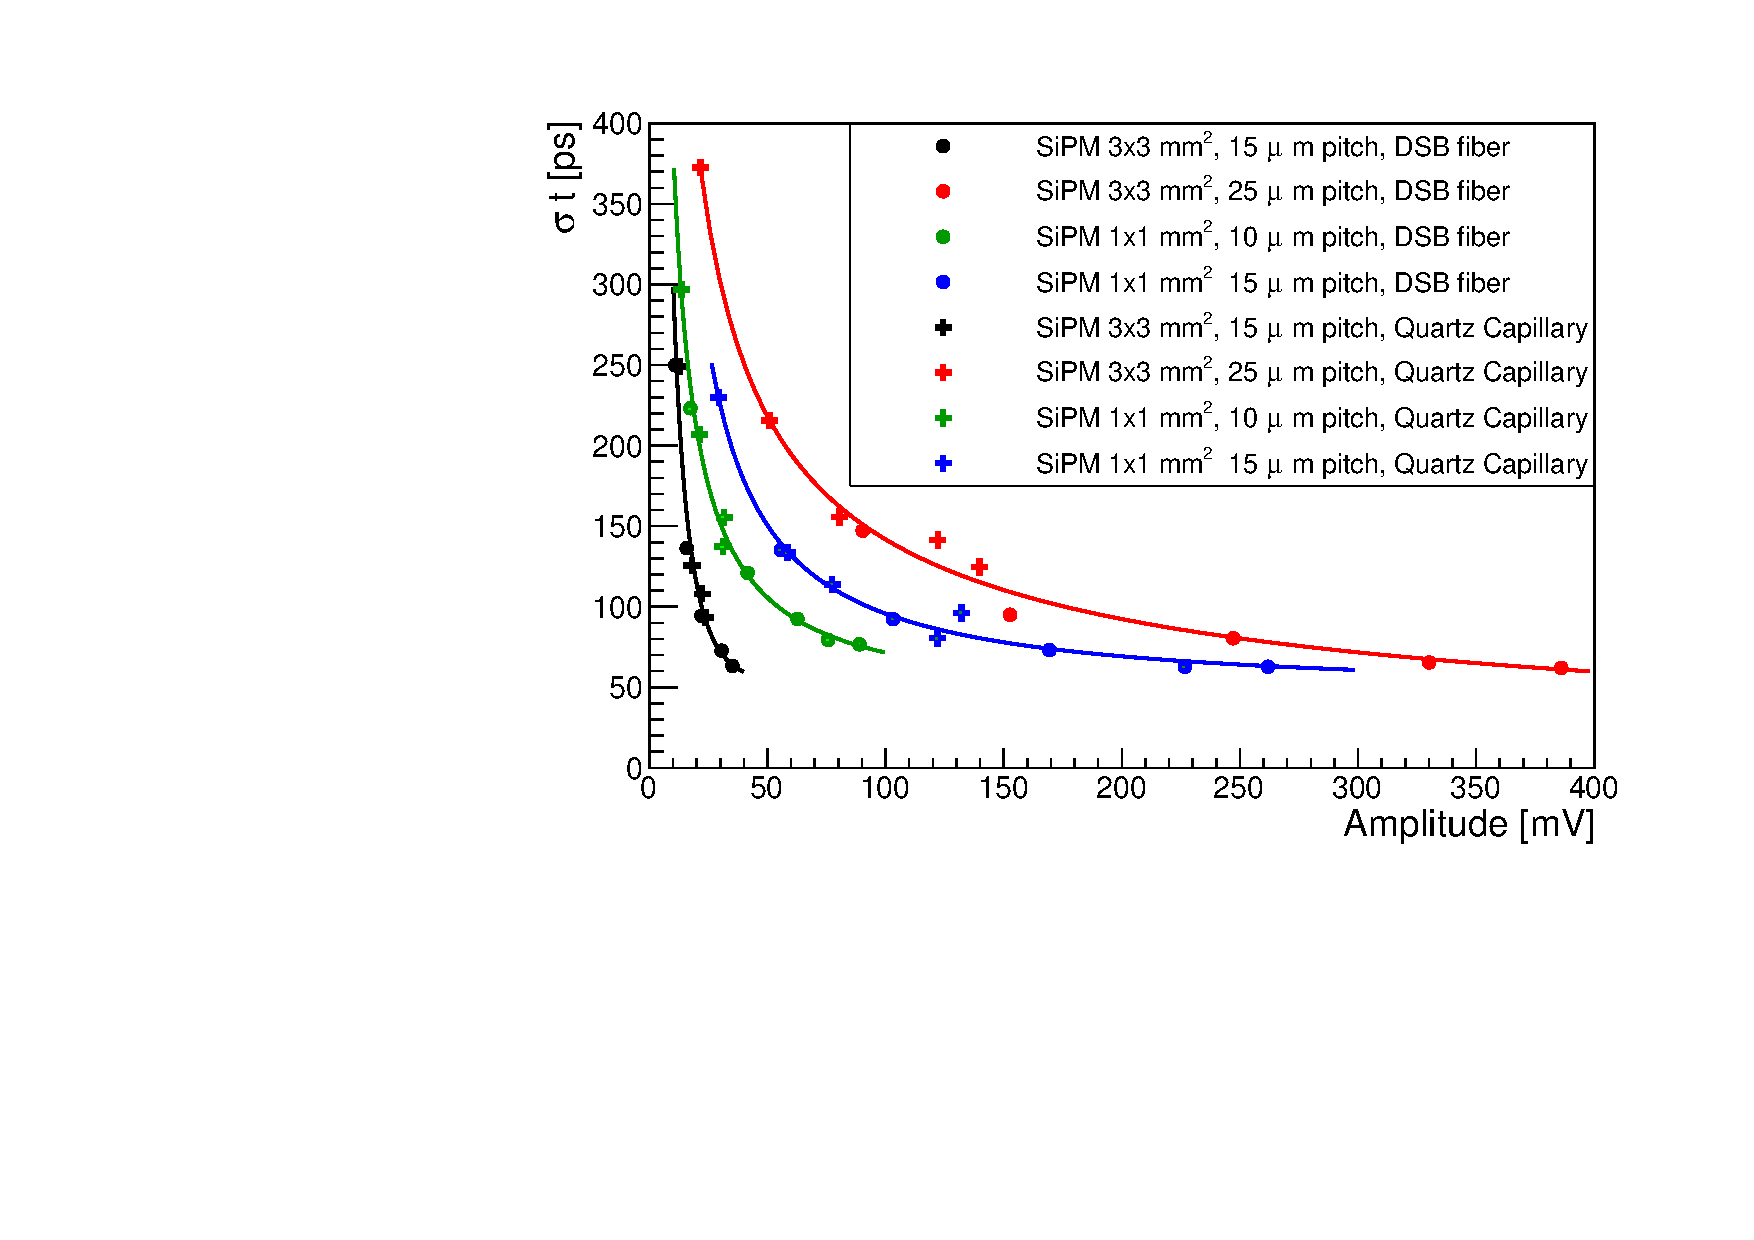
\includegraphics[width=0.99\textwidth]{figures/ShashlikTimeResolution.pdf}
\caption{\label{TimeResolution} The measured time resolution is shown as a
function of the signal amplitude for each individual read-out fiber and SiPM.
The data for each SiPM consists of two sets, one with the DSB WLS plastic fiber
shown as dots and one with the capillaries with a liquid DSB based WLS shown as
squares. }
\end{figure}



As the time measurement precision depends on the rise time of the pulse we also
measure the time resolution as a function of the rise time for signals observed
in the calorimeter cell shown in Figure~\ref{RiseTime}. The rise time of these
signals are driven by the time constants of the wavelength shifter as
demonstrated in reference~\cite{Anderson:2015gha}. For the data presented here,
using SiPMs as photodetectors, we observe that the rise time ranges between
$1.4$~ns and $6$~ns and that the time resolution improves roughly proportional
to the rise time of the signals. In our previous studies of the same calorimeter 
cell using MCPs as photodetectors~\cite{Anderson:2015gha}, the rise time was measured to be around 
$3.0$~ns. The intrinsic rise time for light signals detected by these SiPMs was
measured to be $0.65$~ns using a fast laser described in Sec~\ref{sec:lasertiming} below. 
Additionally, we find that the rise time decreases with increasing amplitude, which was
not observed in our previous studies using MCPs as photodetectors. 
Studies are ongoing to better understand this effect.

\begin{figure}[!htb]
\centering
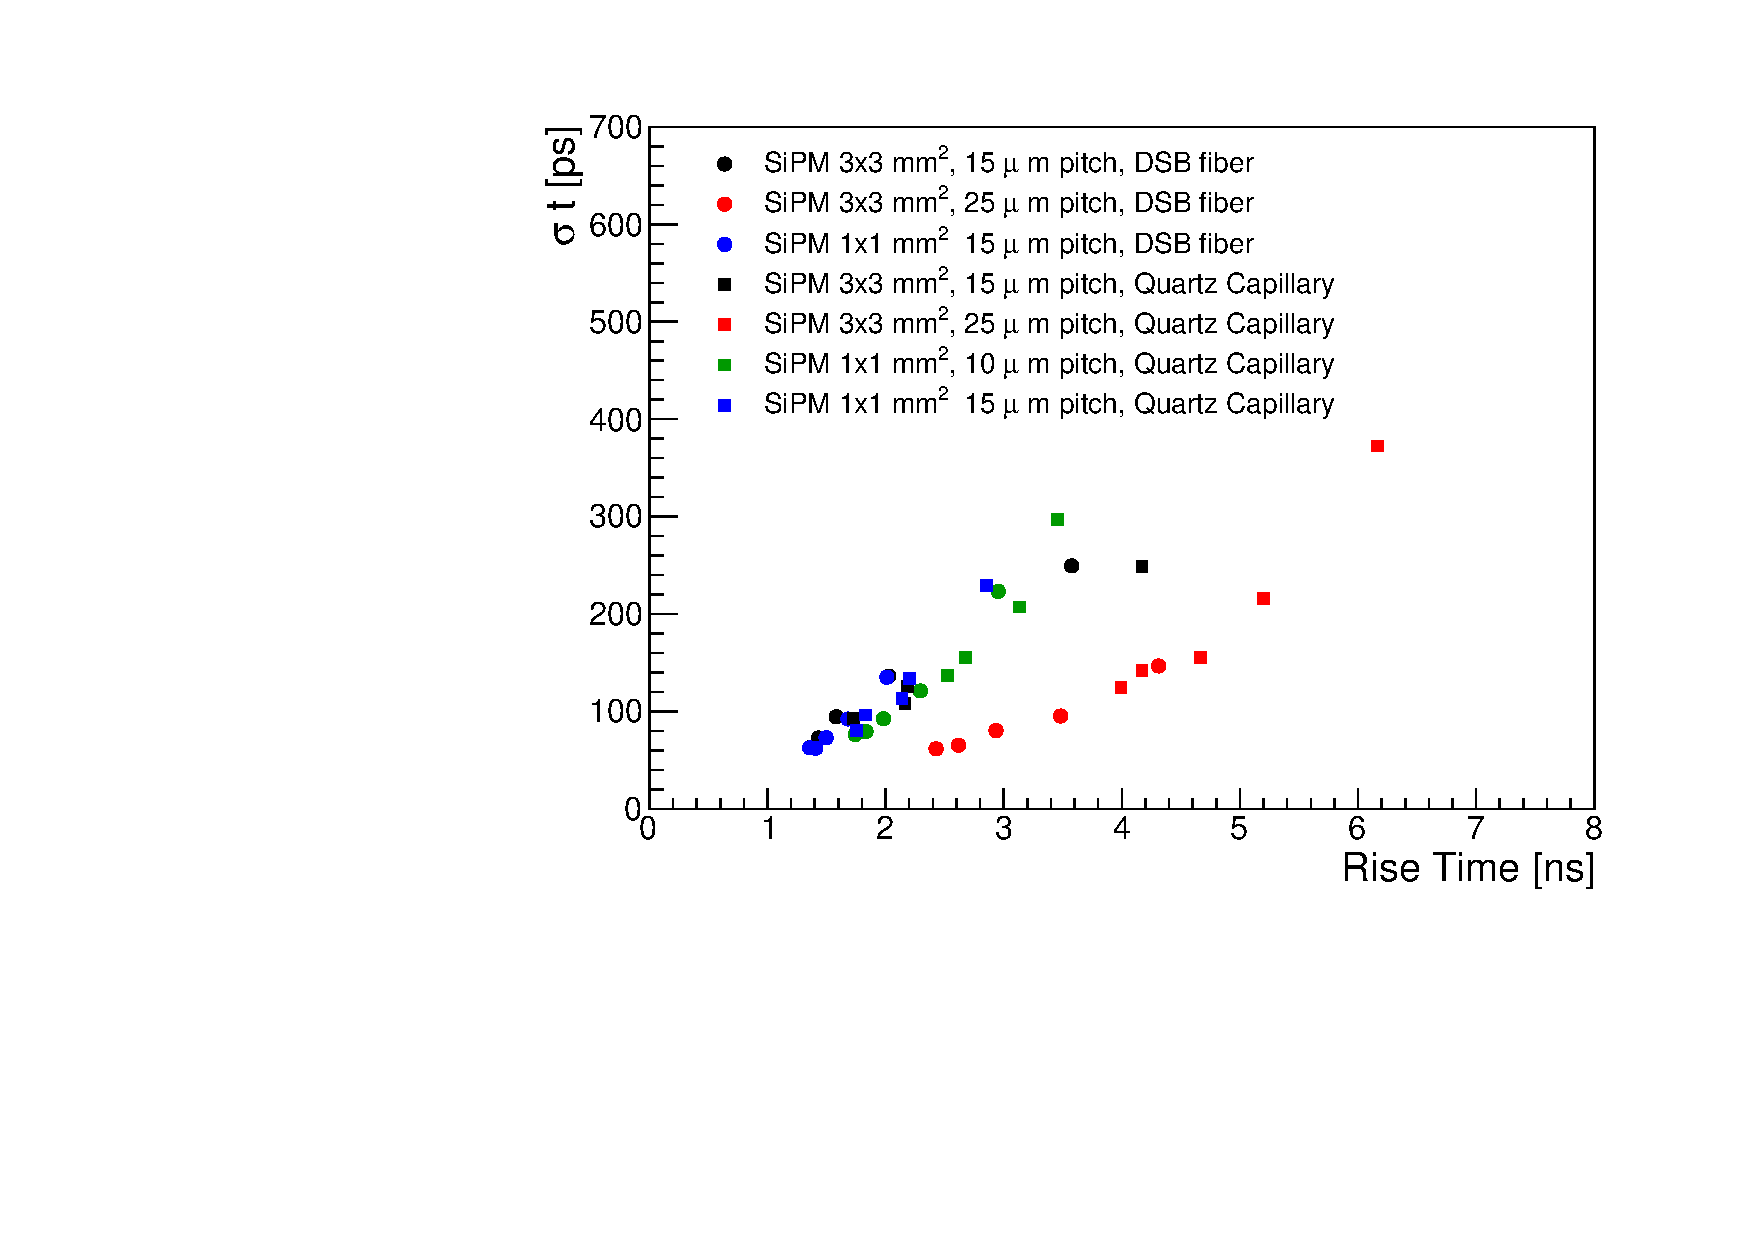
\includegraphics[width=0.99\textwidth]{figures/ShashlikTimeResolutionVsRiseTime.pdf}
\caption{\label{RiseTime}Time resolution is measured as a function of the rise time
for the four different SiPMs. The data recorded with the DSB WLS fibers and the
quartz capillaries are distinguished as dots and squares, respectively. }
\end{figure}

We show the time resolution measured as a function of the beam energy for
signals read out by DSB-doped WLS fibers and quartz capillaries in 
Figure~\ref{TimeResolutionVsEnergy}. Finally, by combining the measured timestamp
from all four SiPM channels, we can significantly improve the time resolution.
The combined time resolution measurements for the DSB WLS fibers and the quartz capillaries 
are shown in Fig~\ref{TimeResolutionCombined} and demonstrate that we can achieve time resolution
of $42$~ps for high energy electromagnetic showers.


\begin{figure}[!htb]
\centering
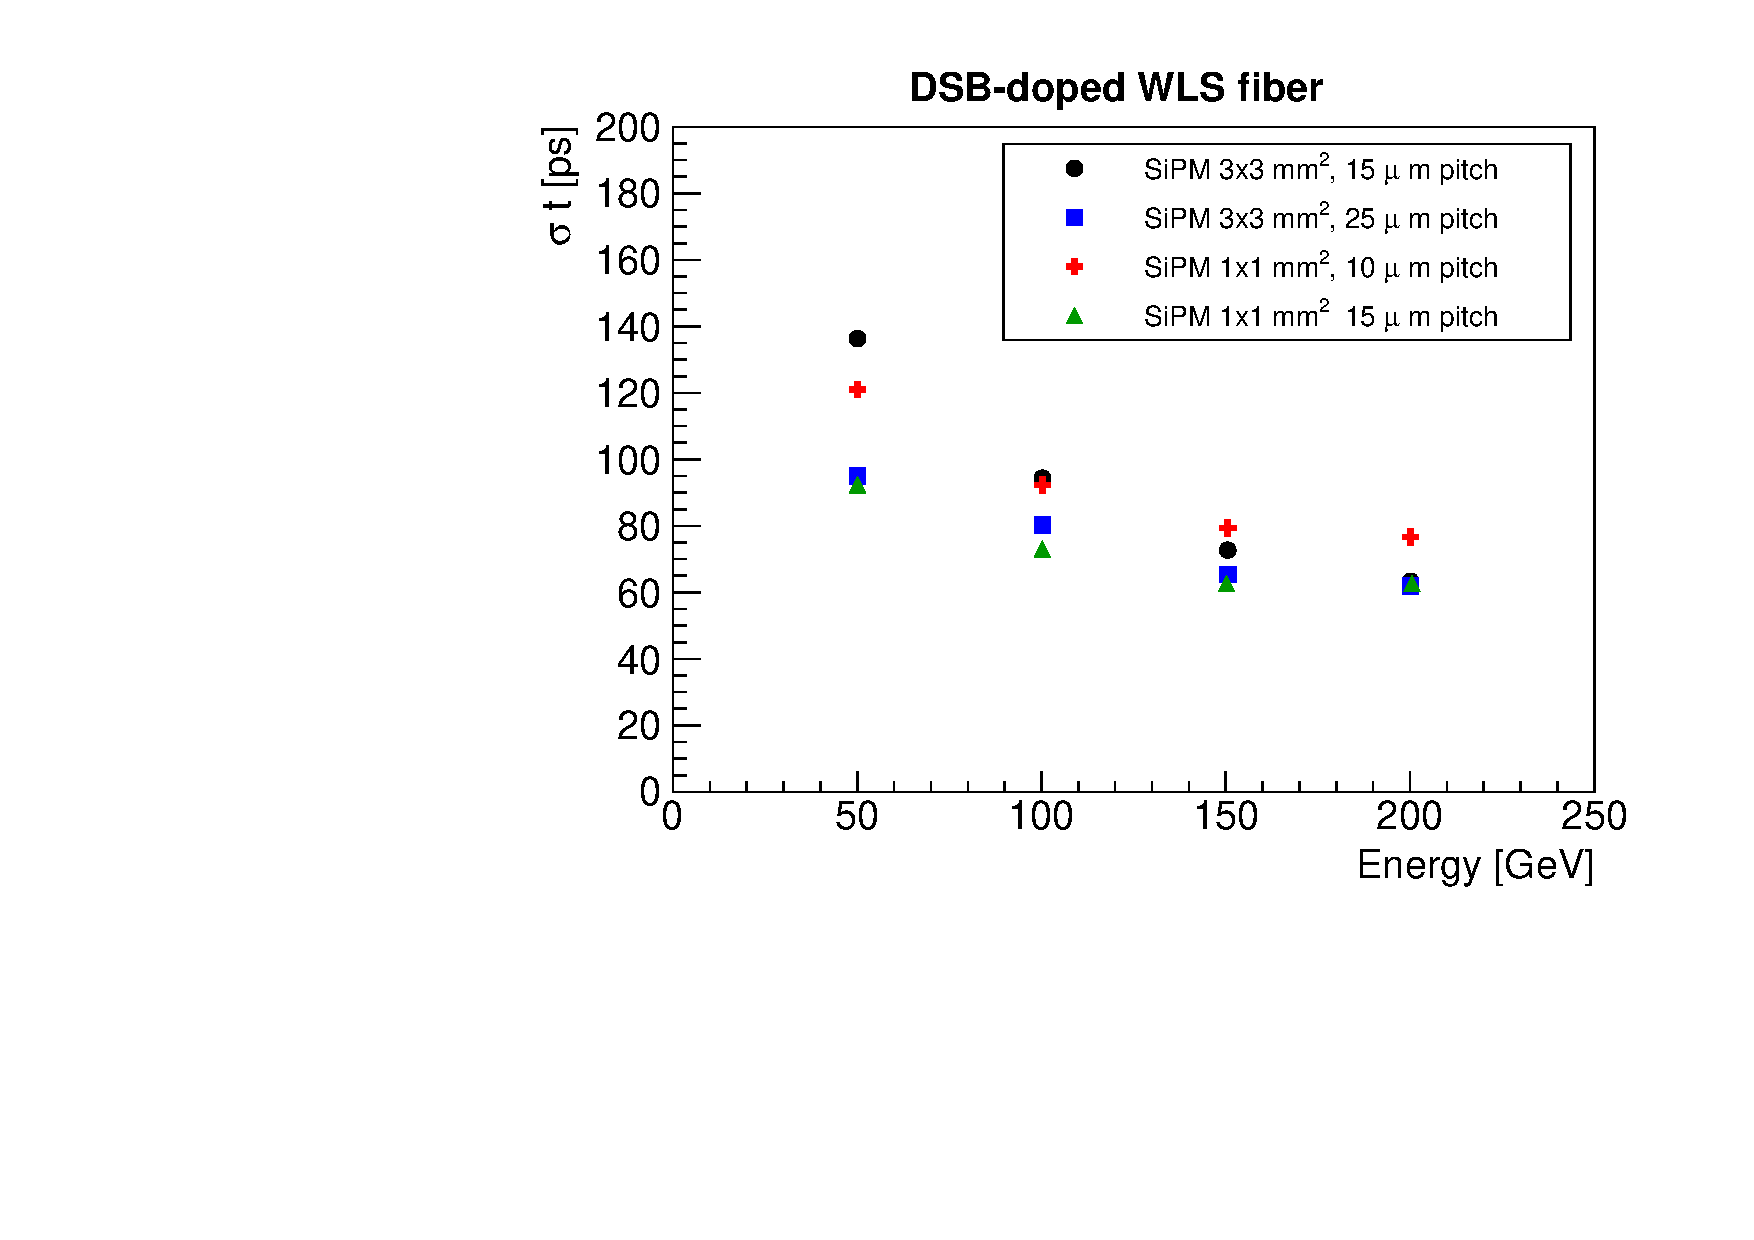
\includegraphics[width=0.49\textwidth]{figures/ShashlikTimeResolutionVsEnergy_DSB.pdf}
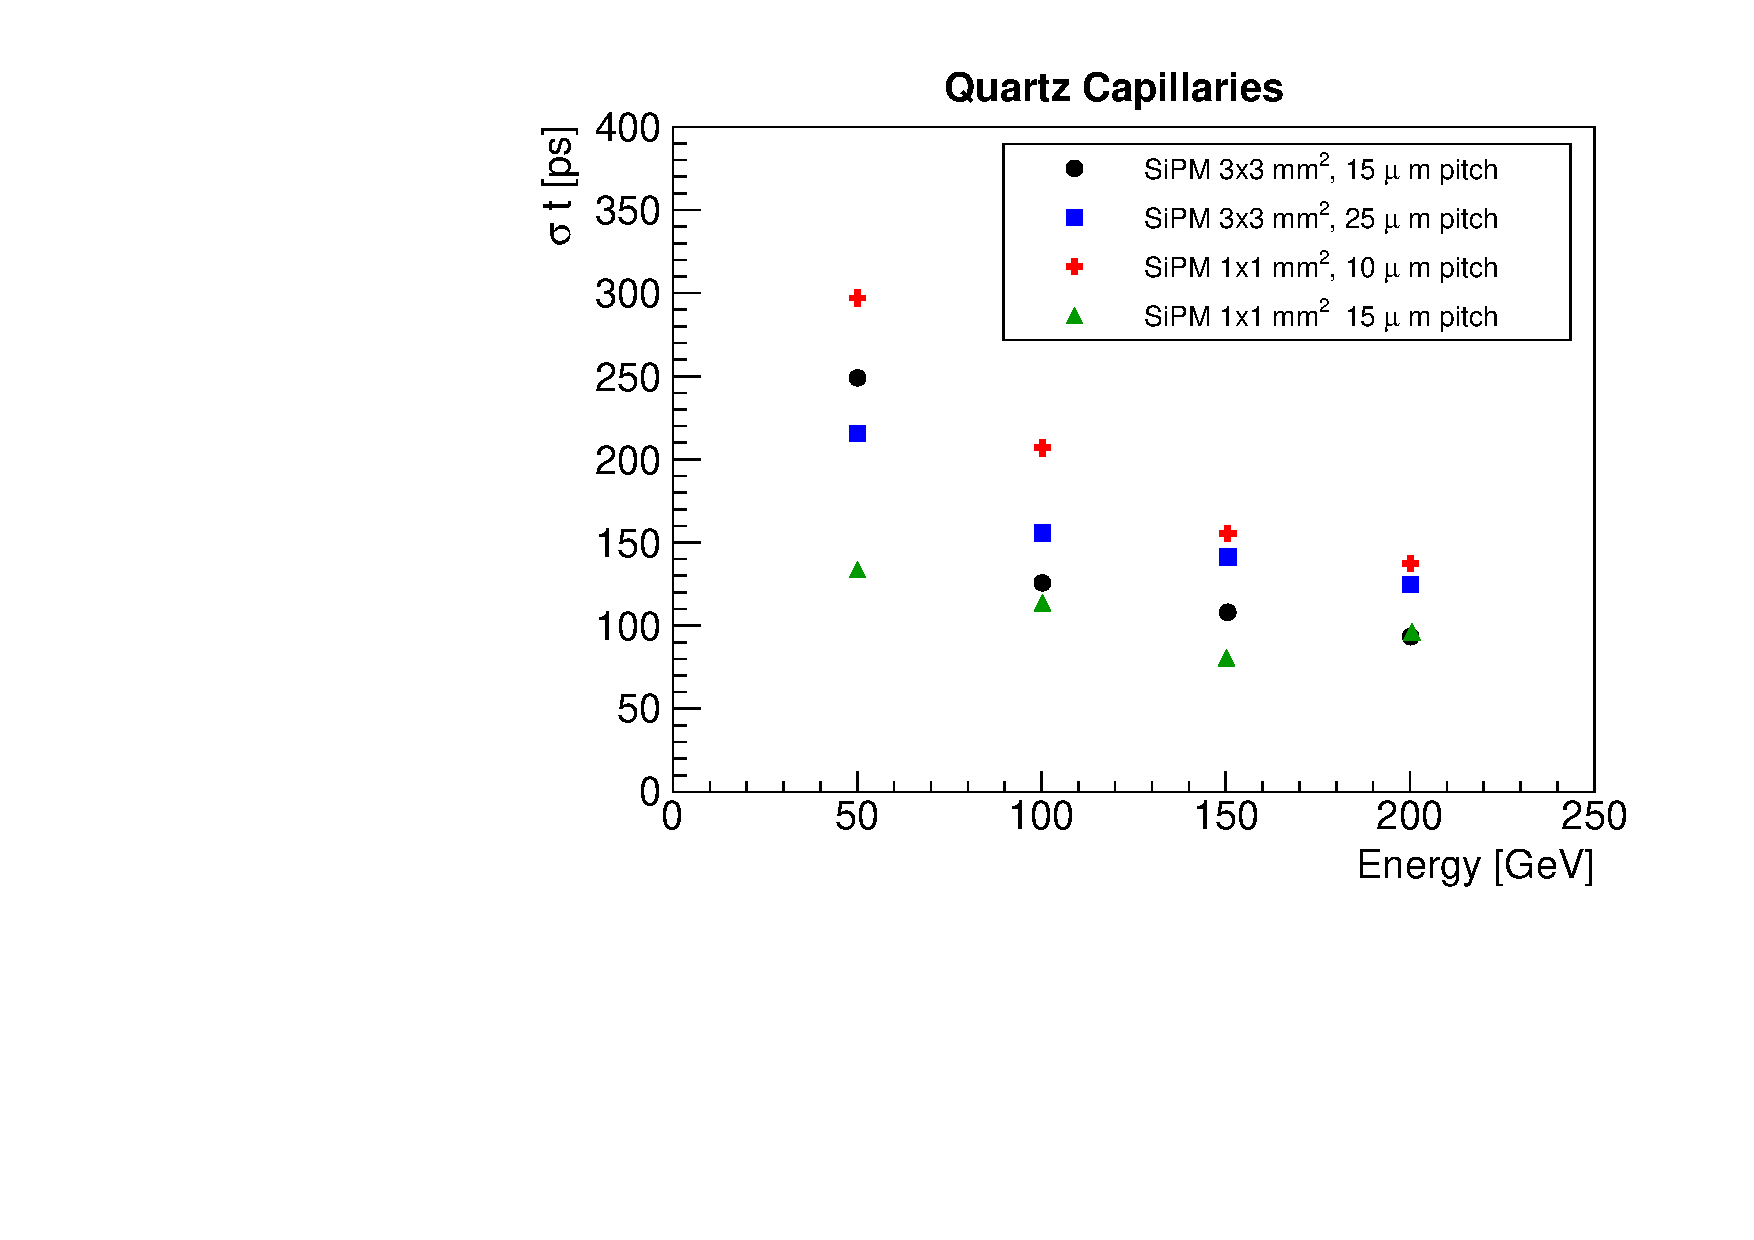
\includegraphics[width=0.49\textwidth]{figures/ShashlikTimeResolutionVsEnergy_Capillaries.pdf}
\caption{\label{TimeResolutionVsEnergy} Time resolution measured in the sampling calorimeter 
cell using the signal of each of the SiPMs individually as a function of the beam energy. 
The data taken using DSB WLS fibers are shown on
the left and the data taken using quartz capillaries are shown on the right}
\end{figure}



\begin{figure}[!htb]
\centering
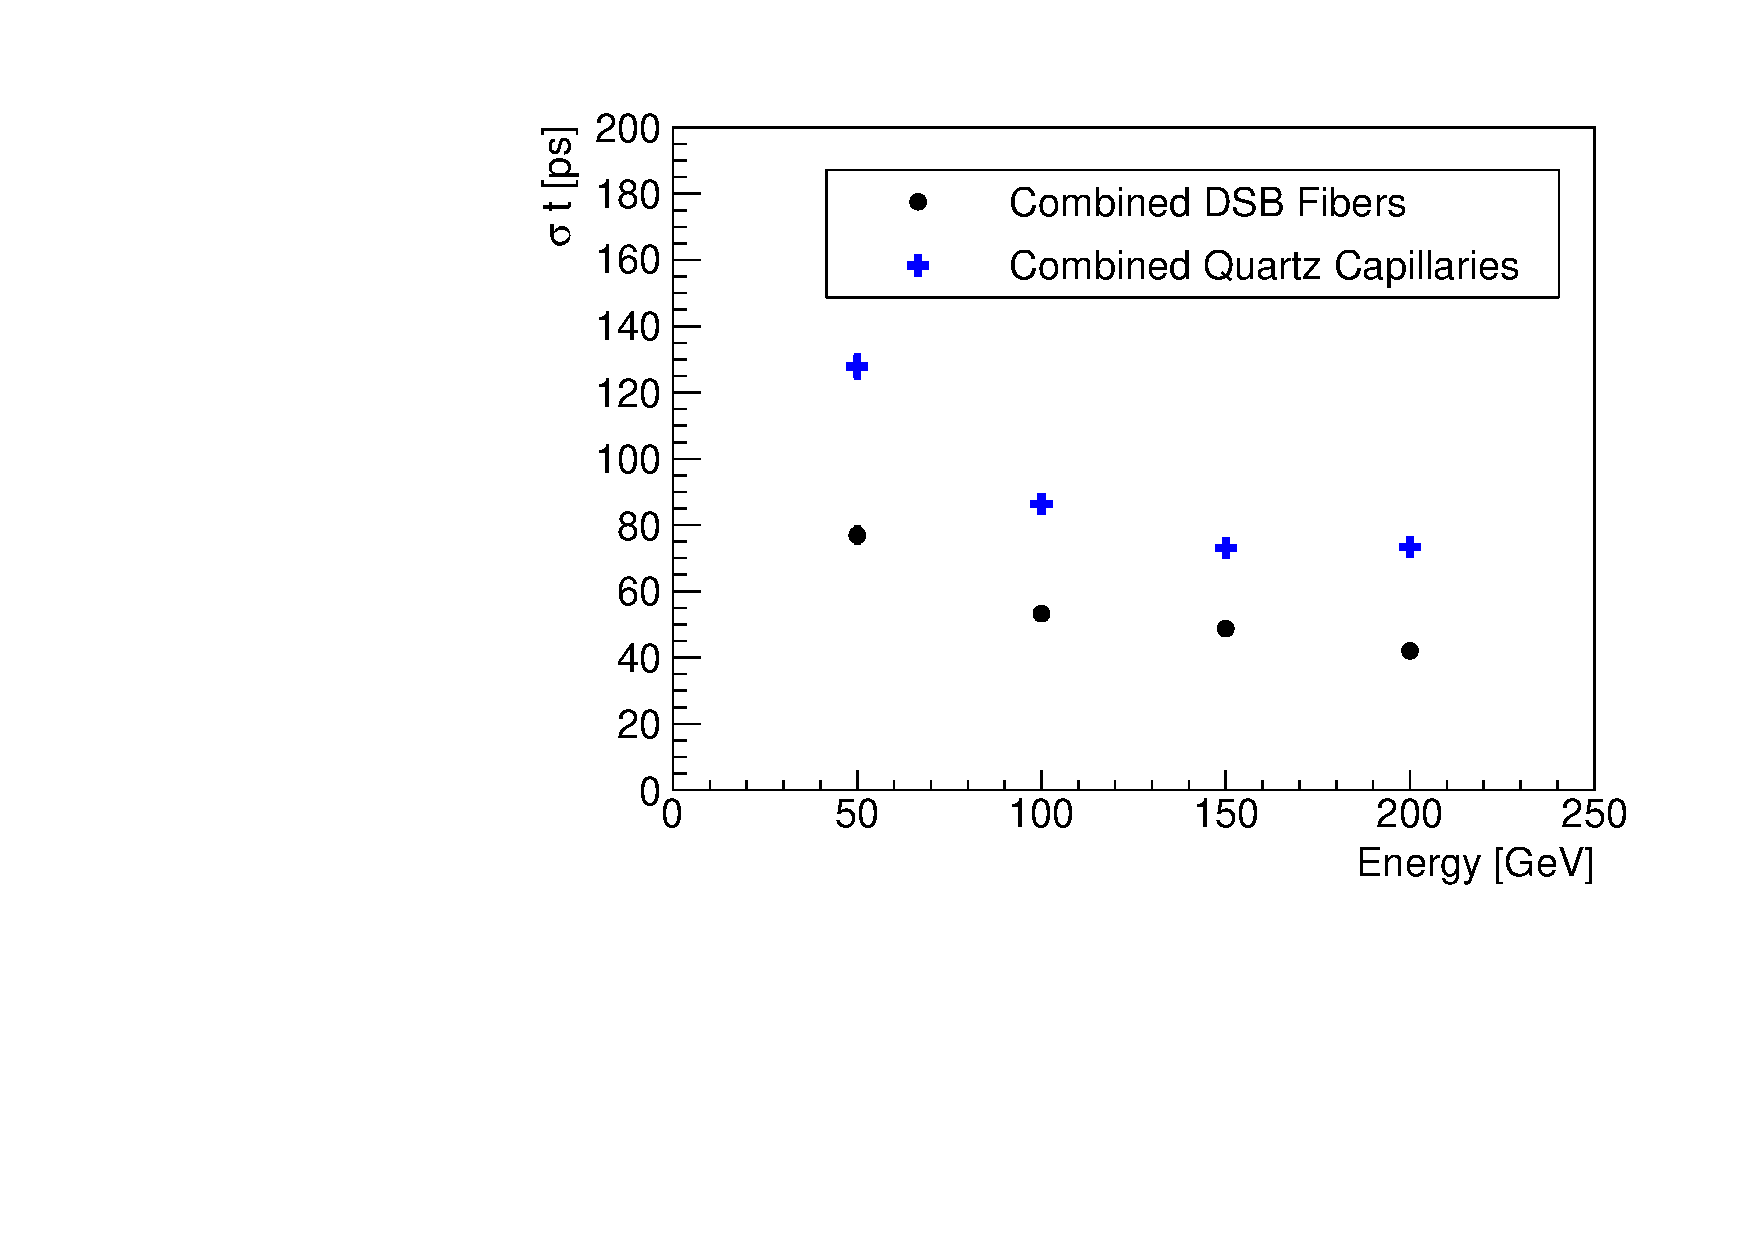
\includegraphics[width=0.8\textwidth]{figures/ShashlikTimeResolutionCombinedChannelVsEnergy.pdf}
\caption{\label{TimeResolutionCombined}  Time resolution measured in the sampling calorimeter cell combining signals from all four  
SiPMs is shown as a function of the beam energy.  The data recorded with the DSB WLS fibers and the
quartz capillaries are distinguished as dots and squares.}
\end{figure}



The light extraction efficiency of capillaries with liquid WLS remains
sufficiently high for dose rates of $100$~Mrad and beyond and for fluences of
$10^{14}$~protons/$\mathrm{cm}^{2}$ and beyond~\cite{shashlik2}. This result
demonstrates the feasibility of achieving good time resolution using a sampling
calorimeter based on LYSO which can survive in dense hadronic collision
environments. The timing performance could be further improved by increasing
the signal size, for example by using larger diameter capillaries or increasing
the calorimeter sampling fraction. 

